%
% Author: Antigoni Kourou
%
\let\textcircled=\pgftextcircled
\chapter{Results}
\label{chap:res}
\section{Overview of sentiment scores}
Sentiment analysis and feature extraction from text reviews of Airbnb feedback system provides us a set of discrete estimators on customers' opinions, referred as sentiment scores. The analysis of these sentiment scores of the chosen dataset reveals that the lowest sentiment score is -0.964 and the highest one is 0.998. Each listing in the dataset has in average 25.1 reviews, each of them containing in average 5.1 sentences. In total there are 12 798 negative sentences (sentiment lower than 0) and 236 904 positive ones, meaning the number of positive sentences is almost 18 times higher than the negative ones.  This fact is supported by Figure \ref{fig:sent}a, which shows the sorted sentiment scores. Then Figure \ref{fig:sent}b shows the normalized frequencies of these sentiment scores rounded by 1. From the graph can be noticed that the most common scores are 0, 0.6 and 0.8, which is firstly supports the argument the most of the scores are highly positive and secondly points out the presence of so many sentences with 0 sentiment, which will be discussed later in this chapter. In addition, it is noticed a tendency of sentiment scores to avoid the "slightly" negative or positive zones around 0, which can have two possible explanations. First, the algorithm may fail in identifying sentences with slight sentiment and second, customers use text reviews to express mostly strong sentiments.
\begin{figure}[h!]
\centering
	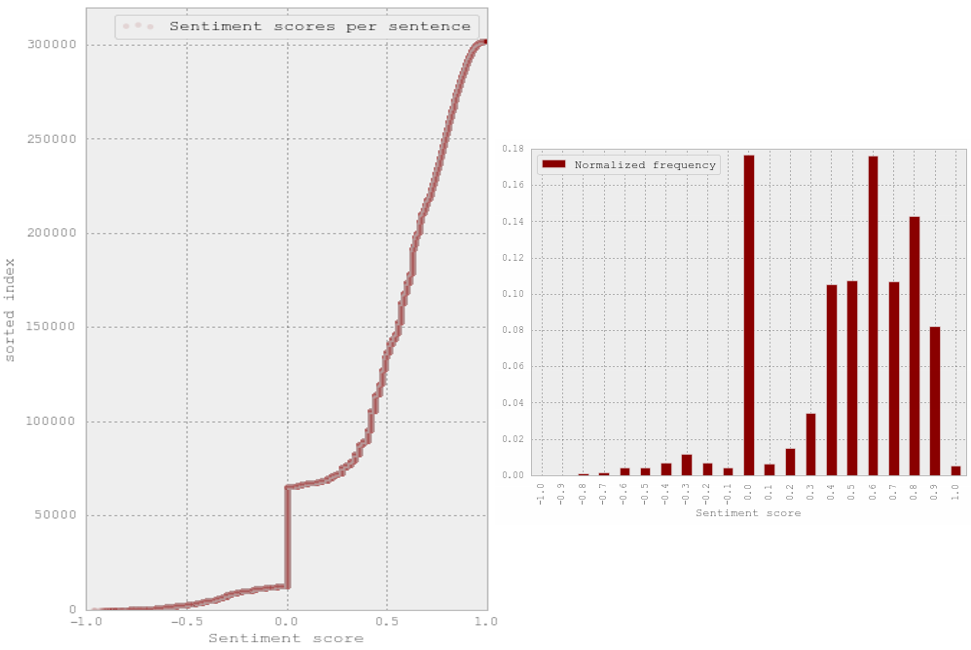
\includegraphics[height=0.35\textheight]{normalized_sentiment_freq}
% * <antigoni.kourou@student.uva.nl> 2016-06-14T10:59:51.526Z:
%
% How to draw a normal distribution curve for the normalized frequencies?
%
% ^.
	\caption{Sentiment scores of each sentence of reviews in the dataset}
	\label{fig:sent}
\end{figure}
The sentiment scores are also grouped by accommodation features and by comparing their distributions of scores to each other and to the overall sentiment scores, it is noticed that the more the feature is mentioned, the more similar its distribution is with the distribution of overall sentiment scores. This part of analysis and visualizations can all be found in Appendix I.
%
% ------------------ NO SENTIMENT -----------------
%
\section{The case of sentences with "no sentiment"}
As it is notices in for graphs of Figure \ref{fig:sent} many sentences have sentiment score equal to 0, meaning neutral sentiment or no-sentiment. From the analysis results 52379 sentences have no-sentiment, consisting in 17.3\% of the total sentences. From the analysis results that a part of these sentences are cases where an automatic cancellation. Every time that the reservation is canceled an automatic message is posted in the text feedback space as a review by the guest-to-be. Therefore without the cases of cancellation, in 16.09 \% of the sentences the pipeline is unable to detect its sentiment, therefore it is seen as neutral. Furthermore from the analysis resulted 1259 cases of cancellations. Their occurrence is checked for each listings and from the analysis we could retrieve the listings which have the highest probability of canceling. It was noticed that in a rare case the number of cancellations reached 27, however the mean number of cancellation would be 1.7 per listing. In total 32.7\% of the listings have canceled at least once the reservation, meaning that the customers should  have to pay attention to the number of cancellations in one listing for making a safe choice. The cases of sentences with sentiment zero are excluded from the following analysis, in order to not affect the average sentiment scores per review or per listing.

\section{Most mentioned features}
An interesting point of view is the analysis of most mentioned feature, which is done in three levels: sentence level, review level and listing level. For all the three levels, we can clearly see that \textit{location} is the most mentioned feature by reviewers of Airbnb and \textit{check-in} is the least mentioned one. From this comparison we can indicate that the frequency of features is more accurate in review level, because we make sure that the opinions of each reviewer are treated equally. Thus, no matter how many times the reviewer mentions the same feature within the review, his/her opinion will generate only one average sentiment score for it. In addition to this argument, measuring the frequencies in sentence level would weight the opinion of some reviewer more than the other. Similarly, in listing level it would take at least one sentence to indicate that the feature is mentioned in the listing, no matter if at one listing it is mentioned 100 times and at another just once, which produces over-estimated frequency values per feature.
\begin{table}[h!]
\footnotesize 
\centering
\begin{tabular}{|m{1.7cm}|m{2.4cm}|m{2.6cm}|m{1.15cm}|}

\hline
\centering {\textbf{}}  & \centering {\textbf{Sentences}} & \centering {\textbf{Reviews}} & {\textbf{Listings}} \\

\hline
\centering {Accuracy}  & \centering {8364} & \centering {7915} &  {1773} \\ \hline

 \centering {Check-in} & \centering {5818} & \centering  {5454} & {1623}\\ \hline
 
 \centering {Cleanliness} & \centering {18440} & \centering {17757} & {2076}\\ \hline
 
\centering  {Communication} & \centering {16894} & \centering {14610} & {2067} \\ \hline

\centering {Location} & \centering {69616} & \centering {44539} & {2331}\\ \hline

\centering {Value} & \centering {19862} & \centering {18811} & {2145}\\ \hline
\end{tabular}
\caption{Number of sentences, reviews and listings where features are mentioned}
\label{res1}
\end{table}

\begin{figure}[h!]
\centering
	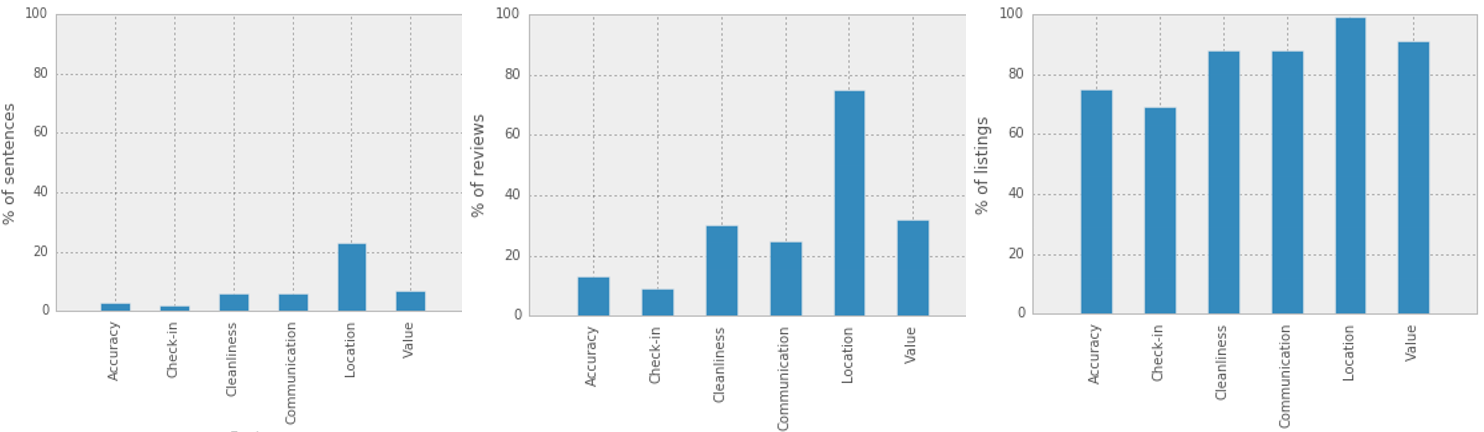
\includegraphics[height=0.2\textheight]{feature_mentioned}
	\caption{Percentage of sentences, reviews and listings where the features are mentioned}
	\label{fig:fea}
\end{figure} 
%
%
%
\section{The trade-off between sentiment and number of reviews}
%
%
\begin{figure}[h!]
	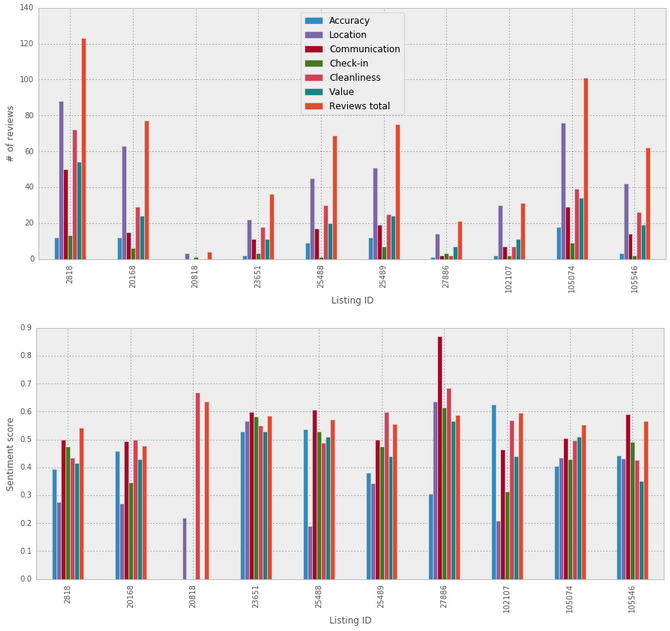
\includegraphics[height=0.67\textheight]{features_sentiment}
	\caption{Features mentioned in review level per each listing and their sentiment}
	\label{fig:feasent}
\end{figure}
Figure \ref{fig:feasent} shows for each feature the number of reviews they are mentioned, as well as the total number of reviews for 10 random listings. In this way, we (as a customer) would prefer to choose listings which have many reviewers talking about a certain feature i.e. \textit{location}, because it makes the sentiment scores more reliable. For each listing the compound sentiment scores of explicit features are easily calculated. The second part of Figure \ref{fig:feasent} shows for the same ten random listings the compound sentiment scores of each feature and the overall sentiment of the listing based in all its reviews. The graphs are placed underneath each other in order for the sentiment scores to be compared with the number of reviews per each feature. From Figure \ref{fig:feasent} we can see that for the listing with ID 22886, even though it has the highest sentiment score on \textit{communication}, only a very few people have commented on it compared to the other listings. Therefore, its high sentiment score is not very reliable. In this case each customer would have to make an individual choice between the listings based on the sentiment of features and their corresponding number of reviews. 

\section{Pipeline ratings compared to Airbnb stars}
An important aspect of analysis is the comparison of pipeline's generated sentiment scores with the Airbnb quantitative data. In the Airbnb feedback system, the customers can see the number of reviews for a listing, the overall average rating after the first three reviews and the average rating of the six specific features: \textit{accuracy, check-in, cleanliness, communication, location, value}. These ratings are compared to the scores generated by the pipeline after converting them into 1-5 stars as mentioned above. The comparison between pipeline generated stars and Airbnb is done for overall ratings and in feature level. 
\subsection{Overall stars per listing}
%
\begin{wrapfigure}[15]{r}{8cm}
\centering
	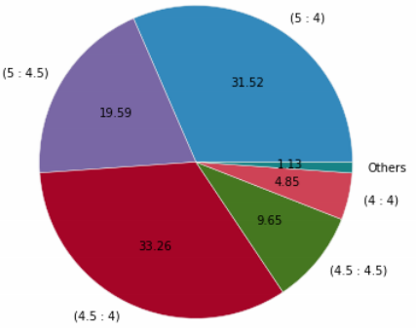
\includegraphics[height=0.27\textheight]{star_combinations}
	\caption{Comparison of combinations Airbnb and pipeline stars per listing}
	\label{fig:comb1}
\end{wrapfigure}
%
From the analysis we can notice that the overall ratings generated from the pipeline are in general quite similar to the ratings in the Airbnb system. Both in Airbnb system and the pipeline results, there is no listing with negative sentiment, lower than 3 stars. All the possible combinations of values are retrieved from the dataset and they are presented in Figure \ref{fig:comb1}. The most common combinations are (5:4),(5:4.5) and (4.5:4), where the first indicator belongs to Airbnb rating and the second to the pipeline. From the combination can be noticed the existence of a systematic tendency of Airbnb ratings to be higher than the ratings generated from the text feedback, concretely in 84.6\% of the cases. These differences are presented in Table \ref{res2}, from where we can indicate that 52.9\% of cases have half a star difference, one star in 31.5\% of cases and only 0.14\% of the cases difference more than one star (3 cases explicitly). 
%
\begin{wraptable}[10]{l}{6.6cm}
\footnotesize 
\centering
\begin{tabular}{|m{1.6cm}||m{1.5cm}|m{1.1cm}|}

\hline
\centering {\textbf{Difference}}  & \centering {\textbf{Frequency}} & {\textbf{\%}} \\

\hline
\centering {\textbf{0.5}}  & \centering {1097}  &  {52.9} \\ \hline

 \centering {\textbf{1.0}} & \centering {654} & {31.5}\\ \hline
 
 \centering {\textbf{0.0}} & \centering {301} & {14.5}\\ \hline
 
\centering  {\textbf{-0.5}} & \centering {17} & {0.8} \\ \hline

\centering {\textbf{1.5}} & \centering {3} & {0.1}\\ \hline

\centering {\textbf{-2.0}} & \centering {1} & {0.04}\\ \hline
\end{tabular}
\centering
\caption{Differences in stars between Airbnb and Pipeline}
\label{res2}
\end{wraptable}

The differences more than 1 stars are treated as isolated cases and they consist of three listings with ID \textit{1357971, 1410370, 2606699}, where Airbnb's ratings are 1.5 stars higher than the pipeline, and only one case of a listing with ID 1022631 where the difference is (-2) stars. For this case, Figure \ref{fig:6.5}, where the difference is the largest, we found out that the listing has actually only one review with one sentence, which has high sentiment score and where the pipeline is based for generating the overall rating.
\begin{figure}[h!]
\centering
	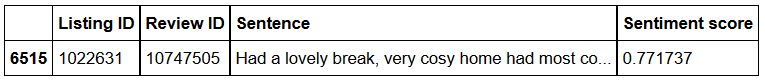
\includegraphics[height=0.07\textheight]{listing-2}
	\caption{Reviews of listing with (-2) stars difference}
	\label{fig:6.5}
\end{figure}
For statistically measuring the differences between values predicted by the pipeline and the  actual Airbnb values, RMSE is used. The RMSE of differences in overall ratings results to be 0.675, meaning that a certain bias exists between the two samples. For its estimation Formula 5.1 is adapted to:
\begin{equation}
RMSE = \sqrt {{\frac{{\sum\limits_{{i = 1}}^n {{{\left( {{y_\textsubscript{i (Airbnb)}} - {{\hat{y}}_\textsubscript{i (Pipeline)}}} \right)}^2}} }}{{n}}}}
\label{RSMEresults}
\end{equation}
%
%
%
\subsection{Stars of features per listing}
\label{6.5.2}
The same comparison as for overall ratings is repeated for each feature. In contrast to the results of overall ratings, the combinations of Airbnb and pipeline stars per feature appear more distributed, new combinations in stars are present and the differences between the predicted stars and Airbnb values are bigger. Table \ref{res3} shows the differences in stars for two features, Accuracy  
%
%
\begin{wraptable}[13]{l}{7.7cm}
\footnotesize 
\centering
\begin{tabular}{|m{0.9cm}|m{0.9cm}|m{0.7cm}||m{0.9cm}|m{0.9cm}|m{0.7cm}|}

\hline
\multicolumn{3}{|c||}{\textbf{Feature:Accuracy}} & \multicolumn{3}{|c|}{\textbf{Feature:Cleanliness}} \\
\hline
\centering {\textbf{Diff.}}  & \centering {\textbf{Freq}} & {\textbf{\%}} & \centering {\textbf{Diff.}}  & \centering {\textbf{Freq}} & {\textbf{\%}}\\

\hline
\centering {\textbf{1.0}}  & \centering {649}  &  {41.2} & \centering {\textbf{0.5}}  & \centering {839}  &  {47.1}\\ \hline

 \centering {\textbf{0.5}} & \centering {571} & {36.9} &  \centering {\textbf{0.0}} & \centering {486} & {27.3}\\ \hline
 
 \centering {\textbf{0.0}} & \centering {162} & {1.4} & \centering {\textbf{1.0}} & \centering {286} & {16.1}\\ \hline
 
\centering {\textbf{1.5}} & \centering {105} & {6.7} & \centering  {\textbf{-0.5}} & \centering {111} & {6.2} \\ \hline

\centering {\textbf{-0.5}} & \centering {32} & {2.1} &  \centering {\textbf{-1.0}} & \centering {27} & {1.5}\\ \hline

\centering {\textbf{2.5}} & \centering {10} & {0.6} &  \centering {\textbf{1.5}} & \centering {22} & {1.2}\\ \hline

 \centering {\textbf{2.0}} & \centering {7} & {0.4} &  \centering {\textbf{2.0}} & \centering {6} & {0.3}\\ \hline
 
\centering  {\textbf{-1.0}} & \centering {6} & {0.3} &  \centering {\textbf{2.5}} & \centering {2} & {0.1} \\ \hline

\centering {\textbf{3.0}} & \centering {5} & {0.3} &  \centering {\textbf{-2.5}} & \centering {1} & {0.05}\\ \hline

\centering {\textbf{3.5}} & \centering {1} & {0.06} &  \centering {\textbf{-1.5}} & \centering {1} & {0.05}\\ \hline
\end{tabular}
\centering
\caption{Differences for two features}
\label{res3}
\end{wraptable}
and Cleanliness. From the table can be seen that for \textit{Cleanliness} the differences are mostly 0.5 stars, but for \textit{Accuracy} difference of 1 stars prevails. From Table \ref{res3} it is also noticed that differences can reach in quite a few cases higher than 1.5, which has two possible explanations. First, the pipeline fails to generate accurate scores per feature and second, the pipeline succeeds in extracting features with negative sentiment, in contrast to Airbnb sytem. In addition to these arguments, the RMSE is calculated for each feature. Its values show that \textit{Location} is the feature with the lowest RMSE 0.48, and \textit{Checkin} is the feature with the highest one 1.51. This results aligns with the fact that \textit{Location} is the most mentioned feature and \textit{Check-in} the least mentioned one (Section 6.2). The comparison of RMSE values leads us to thinking that \textit{the more the feature is mentioned or the more reviews a listing has, the more similar the values of the pipeline are to Airbnb}. Therefore, in order to test this hypothesis, the  number of reviews for the pipeline to generate a rating is limited to 3, the same limit that the Airbnb uses for aggregating the average number of stars. This part of analysis is treated separately in the following section.
\section{Conditional analysis on the number of reviews}
The hypothesis that the number of reviews is reflected in the performance of the pipeline is tested in two levels: for the overall ratings and for each feature. In the first case, the condition set is that a listing must have at least 3 reviews for the pipeline to generate an overall rating. In this case the RMSE changes from 0.675 to 0.673, which is not a significant change. However, the cases with big differences are reduced from 4 to 2. 
On the other hand, in feature level looks like the impact is more significant. The condition in this case is set to "each listing must have the feature \textit{mentioned} in at least three reviews for the pipeline to generate a sentiment score for it". 
\begin{figure}[h!]
\centering
	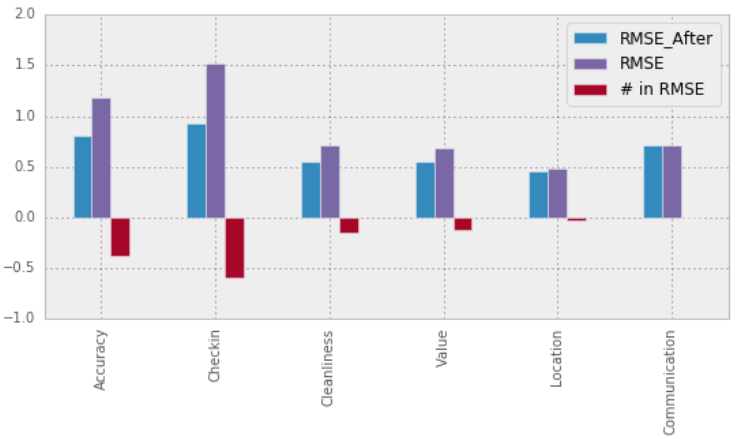
\includegraphics[height=0.4\textheight]{RMSE_features}
	\caption{RMSE per feature before and after setting the condition}
	\label{fig:6.6}
\end{figure}
Figure \ref{fig:6.6} shows the RMSE of differences in Airbnb and the pipeline before and after setting the condition of 3 reviews. The differences are quite significant for \textit{Accuracy} and \textit{Check-in}, which aligns with the features with the smallest number of reviews. Setting this condition makes the analysis of features more reliable and removes biggest the outliers. Figure \ref{fig:6.7} shows how the distribution of the combinations changes after conditioning for these two features. In addition, the analysis showed that 16.5\%  of the listings do not have the sufficient number of reviews to generate a score in feature level. The details of this analysis and the cases of other features can be found in Appendix. 
\begin{figure}[h!]
\centering
	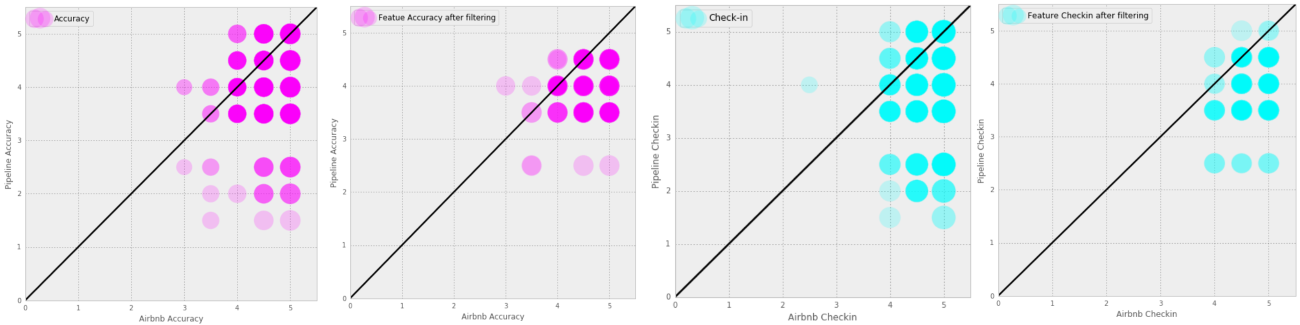
\includegraphics[height=0.19\textheight]{accuracy_checkin}
	\caption{RMSE per feature before and after setting the condition}
	\label{fig:6.7}
\end{figure}

Secondly, from the analysis of star distributions per features as shown above it is noticed that the pipeline identifies features with negative sentiment better than the star rating system of Airbnb. In section \ref{6.5.2} the high RMSE for some features is argued to the a case of outliers or better pipeline results. After conditioning the sentiment scores in 3 or more reviews per feature,
the phenomenon persist, meaning that it is not anymore an error of the pipeline. Some of the cases are investigated closely and they result on true cases where the reviewers negatively comment about features. On the other hand, this result is quite expected as the customers tend to write positive feedback about the listing in general, but explicitly point out the negative elements.
%
%
%
\section{Reducing the bias of Airbnb system}
A few studies suggest text mining as a way of reducing the bias of the star ratings, as reviewers tend to highly rate the listings and only text reviews reveal the negative aspects of a listing \cite{fradkin2016bias,pavlou2006institutional,pavlou2006nature}. In the previous sections we have mentioned the presence of higher rating from Airbnb system than the text reviews and  we have proven that indeed text reviews reveal hidden knowledge about features that the system assigns high ratings. By calculating the mean in differences between the two samples, we suggest that by subtracting half a star from Airbnb values we can retrieve better estimators of stars for a listing, which will both reflect the actual ratings of Airbnb and the ones generated from the text reviews. The RMSE of differences between pipeline and the adjusted sample is 0.357, meaning that the differences are reduced significantly considering that initially RMSE was 0.675. Most importantly the RMSE is comparable with the standard deviation of the sample, which is 0.312. Thus, the values generated by the pipeline are an unbiased estimator of the overall star rating in the Airbnb system. In conclusion, the reduction of Airbnb values with half a star is recommended for retrieving ratings, which consider both manual ratings in the system and the text reviews.
